%========================================
% LESSON CONTENT: Problemas Verbales
%========================================

\lesson{Problemas Verbales}

%========================================
% SECTION 9.1: Introducción
%========================================
\subsectiontitle{Introducción}

Esta lección cubre los siguientes temas importantes:

\begin{itemize}
    \item Traducción de frases verbales a enunciados algebraicos
    \item Establecer ecuaciones partiendo de enunciados verbales
    \item Resolver problemas verbales usando ecuaciones lineales y cuadráticas
    \item Aplicaciones de interés simple y compuesto
\end{itemize}

\medskip

Los problemas verbales representan situaciones de la vida real que pueden modelarse y resolverse usando matemáticas. La clave está en traducir correctamente el lenguaje cotidiano al lenguaje algebraico.

%========================================
% SECTION 9.2: Traducción de Frases
%========================================
\subsectiontitle{Traducción de Frases a Expresiones Algebraicas}

El primer paso para resolver problemas verbales es traducir las frases del problema a expresiones matemáticas.

\begin{definition}
\textbf{Guía para la Traducción:}

\begin{itemize}[leftmargin=*]
    \item \textbf{Variable:} Usa una letra (como $x$, $y$, $n$) para representar la cantidad desconocida.
    \item \textbf{Operaciones:}
    \begin{itemize}
        \item \textbf{Suma (+):} \textit{más que, la suma de, aumentado en, incrementado en}
        \item \textbf{Resta (-):} \textit{menos que, la diferencia de, disminuido en, restado de}
        \item \textbf{Multiplicación ($\cdot$):} \textit{el producto de, veces, multiplicado por, el doble de, el triple de}
        \item \textbf{División ($/$):} \textit{el cociente de, dividido por, la razón de, la mitad de, una tercera parte de}
    \end{itemize}
\end{itemize}
\end{definition}

% Visual representation of operation keywords
\begin{center}
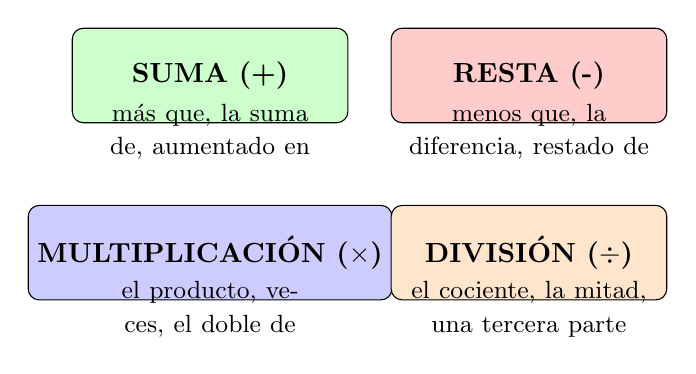
\begin{tikzpicture}[scale=0.9]
    % Suma (Green)
    \node[draw, fill=green!20, minimum width=3.5cm, minimum height=1.2cm, rounded corners] at (0,3)
        {\textbf{SUMA (+)}};
    \node[text width=3.2cm, align=center] at (0,2.2) {\small más que, la suma de, aumentado en};

    % Resta (Red)
    \node[draw, fill=red!20, minimum width=3.5cm, minimum height=1.2cm, rounded corners] at (4.5,3)
        {\textbf{RESTA (-)}};
    \node[text width=3.2cm, align=center] at (4.5,2.2) {\small menos que, la diferencia, restado de};

    % Multiplicación (Blue)
    \node[draw, fill=blue!20, minimum width=3.5cm, minimum height=1.2cm, rounded corners] at (0,0.5)
        {\textbf{MULTIPLICACIÓN ($\times$)}};
    \node[text width=3.2cm, align=center] at (0,-0.3) {\small el producto, veces, el doble de};

    % División (Orange)
    \node[draw, fill=orange!20, minimum width=3.5cm, minimum height=1.2cm, rounded corners] at (4.5,0.5)
        {\textbf{DIVISIÓN ($\div$)}};
    \node[text width=3.2cm, align=center] at (4.5,-0.3) {\small el cociente, la mitad, una tercera parte};
\end{tikzpicture}
\end{center}

\textbf{Ejemplos de Traducción:}

\begin{center}
\begin{tabular}{|l|c|}
\hline
\textbf{Frase} & \textbf{Expresión Algebraica} \\
\hline
un número incrementado en 4 & $x + 4$ \\
\hline
3 más que un número & $x + 3$ \\
\hline
8 menos que un número & $x - 8$ \\
\hline
Un número restado de 10 & $10 - x$ \\
\hline
10 restado de un número & $x - 10$ \\
\hline
el producto de un número y 7 & $7x$ \\
\hline
4 veces un número & $4x$ \\
\hline
Una cuarta parte de un número & $\dfrac{x}{4}$ o $\dfrac{1}{4}x$ \\
\hline
9 más que 4 veces un número & $4x + 9$ \\
\hline
3 menos que tres veces un número y 20 & $3x + 17$ \\
\hline
El doble de un número más 23 & $2x + 23$ \\
\hline
El producto de un número y su triple & $x \cdot 3x = 3x^2$ \\
\hline
Dos enteros consecutivos & $n, n+1$ \\
\hline
\end{tabular}
\end{center}

\begin{example}
\textbf{Ejemplo 1:} Considere la frase ``dos enteros consecutivos''.

\textbf{Solución:}
\begin{itemize}
    \item ¿Puede dar ejemplo de dos enteros consecutivos? Por ejemplo: 5 y 6, o $-3$ y $-2$
    \item Si $n$ representa el menor de dichos números, el entero que le sigue es: $n + 1$
\end{itemize}
\end{example}

\begin{example}
\textbf{Ejemplo 2:} Considere la frase ``la suma de dos números es 17''.

\textbf{Solución:}
\begin{itemize}
    \item Si llamamos $n$ a uno de esos números, el otro número es: $17 - n$
    \item La ecuación sería: $n + (17-n) = 17$
\end{itemize}
\end{example}

\begin{example}
\textbf{Ejemplo 3:} Considere la frase ``la suma de dos enteros consecutivos es 130''.

\textbf{Solución:}
\begin{itemize}
    \item Sea $n$ el primer entero
    \item El entero consecutivo es $n+1$
    \item Expresión algebraica: $n + (n+1) = 130$
\end{itemize}
\end{example}

\begin{example}
\textbf{Ejemplo 4:} El costo de un televisor pequeño es \$47 más que la mitad del costo de un televisor grande.

\textbf{Solución:}
\begin{itemize}
    \item Sea $C$ el costo del televisor grande
    \item La mitad del costo del televisor grande: $\dfrac{C}{2}$
    \item Costo del televisor pequeño: $\dfrac{C}{2} + 47$
\end{itemize}
\end{example}

\begin{example}
\textbf{Ejemplo 5:} María vendió 3 camisetas menos que 4 veces el número de camisetas que vendió su compañero de clase Raúl.

\textbf{Solución:}
\begin{itemize}
    \item Sea $R$ el número de camisetas que vendió Raúl
    \item 4 veces el número de Raúl: $4R$
    \item 3 menos que esa cantidad: $4R - 3$
    \item Número de camisetas que vendió María: $4R - 3$
\end{itemize}
\end{example}

\begin{example}
\textbf{Ejemplo 6:} El costo de un periódico dominical es de 75 centavos.

\textbf{Solución:}
\begin{itemize}
    \item Si $P$ representa el número de periódicos
    \item Cada periódico cuesta \$0.75
    \item Costo total en dólares: $0.75P$ dólares
\end{itemize}
\end{example}

%========================================
% SECTION 9.3: Estrategia General
%========================================
\subsectiontitle{Estrategia General para Resolver Problemas Verbales}

\begin{theorem}
\textbf{Procedimiento de 6 Pasos:}

\begin{enumerate}
    \item \textbf{Leer cuidadosamente el problema.} Hacer un diagrama, dibujo o tabla si es posible.
    \item \textbf{Identificar la cantidad (o cantidades) que el problema pide.} Elija la variable que usará para representar dicha cantidad. \textbf{¡Escríbalo!}
    \item \textbf{Determinar la relación entre cantidades conocidas y la(s) variable(s).} Escriba una ecuación.
    \item \textbf{Resolver la ecuación.}
    \item \textbf{Verificar su(s) solución(es).}
    \item \textbf{Contestar la pregunta original.} Use unidades apropiadas.
\end{enumerate}
\end{theorem}

% Flowchart of problem-solving strategy
\begin{center}
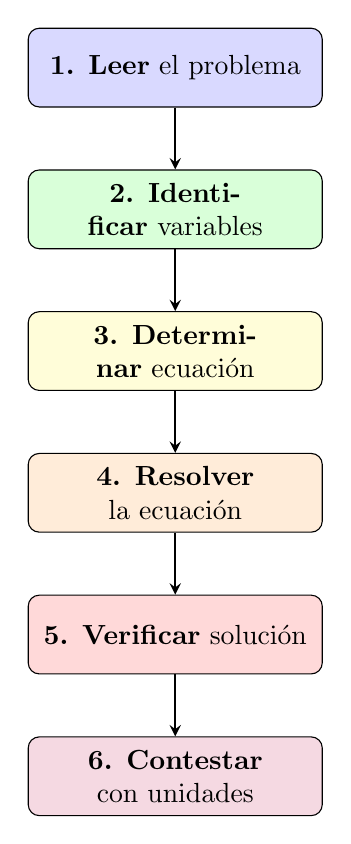
\begin{tikzpicture}[
    stepbox/.style={rectangle, draw, fill=blue!15, text width=3.5cm, text centered, minimum height=1cm, rounded corners},
    arrow/.style={->, thick, >=stealth}
]
    \node[stepbox] (read) at (0,0) {\textbf{1. Leer} el problema};
    \node[stepbox, fill=green!15] (identify) at (0,-1.8) {\textbf{2. Identificar} variables};
    \node[stepbox, fill=yellow!15] (determine) at (0,-3.6) {\textbf{3. Determinar} ecuación};
    \node[stepbox, fill=orange!15] (solve) at (0,-5.4) {\textbf{4. Resolver} la ecuación};
    \node[stepbox, fill=red!15] (verify) at (0,-7.2) {\textbf{5. Verificar} solución};
    \node[stepbox, fill=purple!15] (answer) at (0,-9) {\textbf{6. Contestar} con unidades};

    \draw[arrow] (read) -- (identify);
    \draw[arrow] (identify) -- (determine);
    \draw[arrow] (determine) -- (solve);
    \draw[arrow] (solve) -- (verify);
    \draw[arrow] (verify) -- (answer);
\end{tikzpicture}
\end{center}

%========================================
% SECTION 9.4: Ejemplos Resueltos
%========================================
\subsectiontitle{Ejemplos Resueltos de Problemas Verbales}

\begin{example}
\textbf{Ejemplo 1: Problemas de Números (Suma y Diferencia)}

\textbf{Problema:} Halle dos números cuya suma es 40 y su diferencia es 10.

\textbf{Solución:}
\begin{itemize}
    \item Sea $x$ el número mayor
    \item Sea $y$ el número menor
    \item \textbf{Ecuaciones:}
    \begin{align*}
    x + y &= 40 \quad \text{(la suma es 40)} \\
    x - y &= 10 \quad \text{(la diferencia es 10)}
    \end{align*}
    \item \textbf{Resolver el sistema:}
    \begin{align*}
    \text{De la segunda ecuación: } x &= y + 10 \\
    \text{Sustituir en la primera: } (y + 10) + y &= 40 \\
    2y + 10 &= 40 \\
    2y &= 30 \\
    y &= 15 \\
    x &= 15 + 10 = 25
    \end{align*}
    \item \textbf{Verificación:} $25 + 15 = 40$ \checkmark \quad y \quad $25 - 15 = 10$ \checkmark
    \item \textbf{Respuesta:} Los números son 25 y 15.
\end{itemize}
\end{example}

\begin{example}
\textbf{Ejemplo 2: Problemas con Enteros Consecutivos}

\textbf{Problema:} Halle dos enteros cuyo producto sea 230. Uno de los enteros es tres más que el doble del otro.

\textbf{Solución:}
\begin{itemize}
    \item \textbf{Variables:}
    \begin{itemize}
        \item Sea $n$ un entero.
        \item El otro entero es $2n + 3$.
    \end{itemize}
    \item \textbf{Ecuación:}
    \begin{itemize}
        \item El producto de los dos enteros es 230: $n(2n + 3) = 230$
    \end{itemize}
    \item \textbf{Resolver:}
    \begin{align*}
    2n^2 + 3n &= 230 \\
    2n^2 + 3n - 230 &= 0
    \end{align*}
    Usando la fórmula cuadrática:
    $$n = \frac{-3 \pm \sqrt{9 + 1840}}{4} = \frac{-3 \pm \sqrt{1849}}{4} = \frac{-3 \pm 43}{4}$$
    \begin{align*}
    n &= \frac{40}{4} = 10 \quad \text{o} \quad n = \frac{-46}{4} = -11.5
    \end{align*}
    Como necesitamos enteros, $n = 10$ \\
    El otro entero es $2(10) + 3 = 23$
    \item \textbf{Verificación:} $10 \times 23 = 230$ \checkmark
    \item \textbf{Respuesta:} Los enteros son 10 y 23.
\end{itemize}
\end{example}

\begin{example}
\textbf{Ejemplo 3: Problemas con Edades}

\textbf{Problema:} En 5 años, Miguel tendrá 3 veces más que la edad que tenía hace 7 años. ¿Cuántos años tiene ahora?

\textbf{Solución:}
\begin{itemize}
    \item Sea $x$ = edad actual de Miguel
    \item \textbf{Ecuación:}
    \begin{itemize}
        \item Edad en 5 años: $x + 5$
        \item Edad hace 7 años: $x - 7$
        \item $(x + 5) = 3(x - 7)$
    \end{itemize}
    \item \textbf{Resolver:}
    \begin{align*}
    x + 5 &= 3x - 21 \\
    5 + 21 &= 3x - x \\
    26 &= 2x \\
    x &= 13
    \end{align*}
    \item \textbf{Verificación:}
    \begin{itemize}
        \item En 5 años tendrá: $13 + 5 = 18$ años
        \item Hace 7 años tenía: $13 - 7 = 6$ años
        \item ¿Es 18 tres veces 6? $3 \times 6 = 18$ \checkmark
    \end{itemize}
    \item \textbf{Respuesta:} Miguel tiene 13 años ahora.
\end{itemize}
\end{example}

\begin{example}
\textbf{Ejemplo 4: Problemas de Comisiones}

\textbf{Problema:} Luis es vendedor de bicicletas y recibe un sueldo base más comisiones. Su salario mensual es de \$300 y recibe una comisión de \$15 por cada bicicleta que vende. ¿Cuántas bicicletas tiene que vender en un mes para tener un ingreso mensual de \$750?

\textbf{Solución:}
\begin{itemize}
    \item Sea $x$ = número de bicicletas vendidas
    \item \textbf{Ecuación:}
    \begin{itemize}
        \item Ingreso total = sueldo base + comisiones
        \item $750 = 300 + 15x$
    \end{itemize}
    \item \textbf{Resolver:}
    \begin{align*}
    750 - 300 &= 15x \\
    450 &= 15x \\
    x &= 30
    \end{align*}
    \item \textbf{Verificación:} $300 + 15(30) = 300 + 450 = 750$ \checkmark
    \item \textbf{Respuesta:} Luis debe vender 30 bicicletas.
\end{itemize}
\end{example}

\begin{example}
\textbf{Ejemplo 5: Problemas de Promedios}

\textbf{Problema:} Las puntuaciones obtenidas por José en tres exámenes de matemáticas son 85, 98, 87. Determine la puntuación que debe obtener en un cuarto examen para que su promedio sea de 90.

\textbf{Solución:}
\begin{itemize}
    \item Sea $x$ = puntuación en el cuarto examen
    \item \textbf{Ecuación:}
    \begin{itemize}
        \item Promedio = $\dfrac{\text{suma de puntuaciones}}{\text{número de exámenes}}$
        \item $90 = \dfrac{85 + 98 + 87 + x}{4}$
    \end{itemize}
    \item \textbf{Resolver:}
    \begin{align*}
    90 &= \frac{270 + x}{4} \\
    360 &= 270 + x \\
    x &= 90
    \end{align*}
    \item \textbf{Verificación:} $\dfrac{85 + 98 + 87 + 90}{4} = \dfrac{360}{4} = 90$ \checkmark
    \item \textbf{Respuesta:} José debe obtener 90 puntos en el cuarto examen.
\end{itemize}
\end{example}

%========================================
% SECTION 9.5: Aplicaciones Financieras
%========================================
\subsectiontitle{Aplicaciones Financieras}

\begin{definition}
\textbf{Vocabulario Financiero:}
\begin{itemize}
    \item \textbf{Intereses:} dinero que se nos paga (o cobra) por nuestros ahorros (o préstamos)
    \item \textbf{Capital (o principal):} cantidad de dinero que ahorro (o tomo prestado) del banco
    \item \textbf{Tasa de interés:} se define como un porcentaje del principal. A menos que se indique lo contrario, la tasa de interés es anual.
\end{itemize}
\end{definition}

\textbf{Cantidad Acumulada:}

La cantidad acumulada, $A$, en el banco luego de una inversión de $P$ dólares por un tiempo de $t$ años, y que ha ganado intereses, $I$, se puede expresar en general:

$$A = P + I$$

\textbf{Ejemplo:} Si ahorré $P = \$3000$ y gané $I = \$190$, entonces acumulé $A = \$3190$.

\subsubsection*{Interés Simple}

\begin{definition}
\textbf{Interés Simple:} Interés que se calcula solamente sobre el principal, y se paga anualmente.

$$I = Prt$$

donde:
\begin{itemize}
    \item $I$ = interés simple
    \item $P$ = principal (capital)
    \item $r$ = tasa de interés (en decimal)
    \item $t$ = tiempo en años
\end{itemize}
\end{definition}

\newpage

\begin{example}
\textbf{Ejemplo de Interés Simple (1 año)}

\textbf{Problema:} Se invierten \$2000 a un interés simple de 9.5\% anual.
\begin{enumerate}[label=\alph*)]
    \item Calcule el interés ganado al cabo de un año.
    \item ¿Cuál es la cantidad acumulada al final del año?
\end{enumerate}

\textbf{Solución:}

a) Usamos la fórmula de interés simple:
\begin{itemize}
    \item $P = 2000$, $r = 0.095$, $t = 1$
    \item $I = Prt = (2000)(0.095)(1) = \$190$
\end{itemize}

b) Al final del año se tienen:
\begin{itemize}
    \item $A = P + I = 2000 + 190 = \$2190$
\end{itemize}
\end{example}

\begin{example}
\textbf{Ejemplo de Interés Simple (meses)}

\textbf{Problema:} Se invierten \$3500 a un interés simple de 7.5\% anual. Calcule el interés ganado al cabo de 8 meses.

\textbf{Solución:}
\begin{itemize}
    \item $P = 3500$, $r = 0.075$, $t = \dfrac{8}{12} = \dfrac{2}{3}$ años
    \item $I = Prt = (3500)(0.075)\left(\dfrac{2}{3}\right)$
    \item $I = (3500)(0.075)(0.6667) = \$175$
\end{itemize}

\textbf{Respuesta:} El interés ganado es \$175.
\end{example}

\newpage
\subsubsection*{Interés Compuesto}

Cuando el capital se invierte utilizando interés compuesto, el banco paga intereses varias veces al año. Cada instancia en la que se paga interés, se toma en cuenta los intereses que se van acumulando y los balances correspondientes.

\begin{definition}
\textbf{Fórmula del Interés Compuesto:}

La cantidad acumulada, $A$, por la inversión de $P$ dólares usando interés compuesto:

$$A = P\left(1 + \frac{r}{m}\right)^{mt}$$

donde:
\begin{itemize}
    \item $m$ = número de veces que nos pagan intereses al año
    \item $r$ = tasa de interés anual (en decimal)
    \item $t$ = tiempo en años
    \item $P$ = principal
\end{itemize}
\end{definition}

\textbf{Valores que toma $m$:}

\begin{center}
\begin{tabular}{|c|c|}
\hline
\textbf{Término} & $\mathbf{m}$ \\
\hline
anualmente & 1 \\
\hline
semestralmente & 2 \\
\hline
trimestralmente & 4 \\
\hline
mensualmente & 12 \\
\hline
diariamente & 365 \\
\hline
\end{tabular}
\end{center}

\begin{example}
\textbf{Ejemplo de Interés Compuesto Mensualmente}

\textbf{Problema:} Si se invierten \$3000 a tasa de interés de 4\% anual compuesto mensualmente, encuentre la cantidad acumulada luego de:
\begin{enumerate}[label=\alph*)]
    \item 20 años
    \item 6 meses
\end{enumerate}

\textbf{Solución:}

a) Para 20 años:
\begin{itemize}
    \item $P = 3000$, $r = 0.04$, $m = 12$, $t = 20$
    \item $A = 3000\left(1 + \dfrac{0.04}{12}\right)^{12 \times 20}$
    \item $A = 3000(1.003333)^{240}$
    \item $A = 3000(2.2255)$
    \item $A \approx \$6676.50$
\end{itemize}

b) Para 6 meses:
\begin{itemize}
    \item $t = \dfrac{6}{12} = 0.5$ años
    \item $A = 3000\left(1 + \dfrac{0.04}{12}\right)^{12 \times 0.5}$
    \item $A = 3000(1.003333)^{6}$
    \item $A = 3000(1.0202)$
    \item $A \approx \$3060.60$
\end{itemize}
\end{example}

\begin{example}
\textbf{Ejemplo de Interés Compuesto Trimestralmente}

\textbf{Problema:} Si se invierten \$1000 a una tasa de interés compuesto de 4.5\%, encuentra la cantidad acumulada luego de dos años si se computa el interés trimestralmente.

\textbf{Solución:}
\begin{itemize}
    \item $P = 1000$, $r = 0.045$, $m = 4$, $t = 2$
    \item $A = 1000\left(1 + \dfrac{0.045}{4}\right)^{4 \times 2}$
    \item $A = 1000(1.01125)^{8}$
    \item $A = 1000(1.0932)$
    \item $A \approx \$1093.20$
\end{itemize}

\textbf{Respuesta:} La cantidad acumulada es aproximadamente \$1093.20.
\end{example}

% Visual comparison of Simple vs Compound Interest
\begin{center}
\begin{tikzpicture}
    % Simple Interest box
    \node[draw, fill=blue!10, text width=6cm, minimum height=2cm, rounded corners] at (0,0) {
        \textbf{Interés Simple} \\[0.3cm]
        $I = Prt$ \\[0.2cm]
        \small Se calcula solo sobre el principal
    };

    % Compound Interest box
    \node[draw, fill=green!10, text width=6cm, minimum height=2cm, rounded corners] at (0,-3) {
        \textbf{Interés Compuesto} \\[0.3cm]
        $A = P\left(1 + \dfrac{r}{m}\right)^{mt}$ \\[0.2cm]
        \small Se calcula sobre el principal + intereses acumulados
    };
\end{tikzpicture}
\end{center}

\textbf{Notas Importantes:}
\begin{itemize}
    \item Siempre defina claramente sus variables antes de establecer ecuaciones
    \item Verifique sus respuestas sustituyendo en el problema original
    \item Asegúrese de que sus respuestas tengan sentido en el contexto del problema
    \item Use unidades apropiadas en sus respuestas finales
    \item Para problemas de interés, recuerde convertir porcentajes a decimales
    \item Para problemas de tiempo, asegúrese de que todas las unidades sean consistentes (años, meses, días)
\end{itemize}
